\documentclass[tikz,border=5pt]{standalone}

\usepackage{tkz-euclide}
\usepackage{amsmath}

\begin{document}

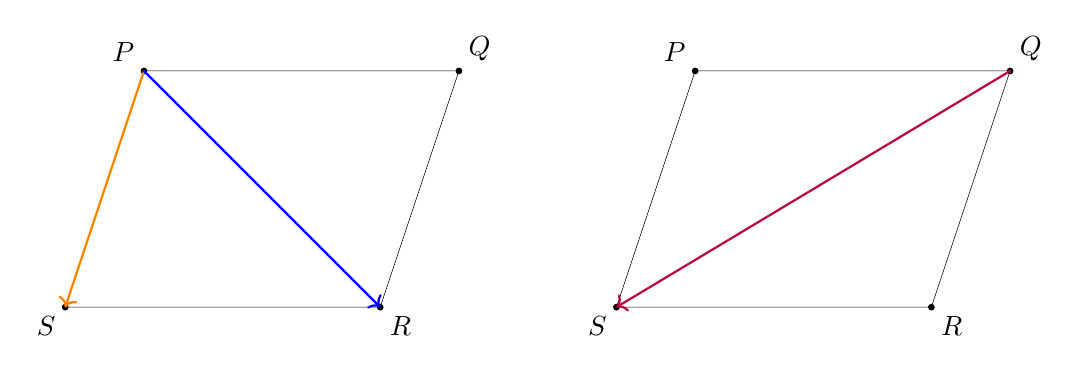
\begin{tikzpicture}

% -----------------------
% Points du parallélogramme
% -----------------------
\coordinate (P) at (0,0);
\coordinate (Q) at (4,0);
\coordinate (S) at (-1,-3);
\coordinate (R) at ($(Q)+(S)-(P)$);

% -----------------------
% Figure
% -----------------------
\tkzDrawPolygon(P,Q,R,S)

% -----------------------
% Labels
% -----------------------
\tkzLabelPoints[above left](P)
\tkzLabelPoints[above right](Q)
\tkzLabelPoints[below left](S)
\tkzLabelPoints[below right](R)
\tkzDrawPoints[color=black,size=2](P,...,S)

% -----------------------
% Vecteurs directionnels
% -----------------------
\tkzDrawSegment[->,orange,thick](P,S)

\tkzDrawSegment[->,blue,thick](P,R)

%\tkzDrawSegment[->,purple,thick](Q,S)

\begin{scope}[xshift=7cm]
   % -----------------------
% Points du parallélogramme
% -----------------------
\coordinate (P) at (0,0);
\coordinate (Q) at (4,0);
\coordinate (S) at (-1,-3);
\coordinate (R) at ($(Q)+(S)-(P)$);

% -----------------------
% Figure
% -----------------------
\tkzDrawPolygon(P,Q,R,S)

% -----------------------
% Labels
% -----------------------
\tkzLabelPoints[above left](P)
\tkzLabelPoints[above right](Q)
\tkzLabelPoints[below left](S)
\tkzLabelPoints[below right](R)
\tkzDrawPoints[color=black,size=2](P,...,S)

% -----------------------
% Vecteurs directionnels
% -----------------------
%\tkzDrawSegment[->,orange,thick](P,S)

%\tkzDrawSegment[->,blue,thick](P,R)

\tkzDrawSegment[->,purple,thick](Q,S)

 
\end{scope}

\end{tikzpicture}

\end{document}